\section{Dataset Exploration}\label{dataset_exploration}

The dataset, referred to as \texttt{dataset\_19}, comprises a collection of MRI images organized into four subfolders, each representing a distinct class of brain tumors. Each subfolder contains 120 images, resulting in a well-balanced dataset with a total of 480 images. This balance is essential for training deep learning models, as it mitigates the risk of bias towards any particular class, ensuring that the model learns to distinguish among all categories effectively.

The dataset includes images representing four types of brain tumors: glioma, meningioma, pituitary tumors, and cases with no tumors. Specifically, it consists of 120 images of glioma tumors, 120 images of meningioma tumors, 120 images of pituitary tumors, and 120 images with no tumors.

Each image in the dataset captures the brain from different perspectives, including axial, coronal, and sagittal views. These diverse views are crucial as they provide comprehensive information about the tumor's location, size, and relation to surrounding structures. Axial views offer a horizontal slice of the brain, coronal views provide a frontal slice, and sagittal views give a side slice. Including these various perspectives ensures that the model can learn robust features and improve its ability to generalize across different cases.

The distribution of images across these classes is depicted in Figure \ref{fig:data_distribution}. This visual representation underscores the dataset's balance and uniformity, further highlighting its suitability for developing a deep learning model for brain tumor classification.

\begin{figure}[H]
  \begin{center}
    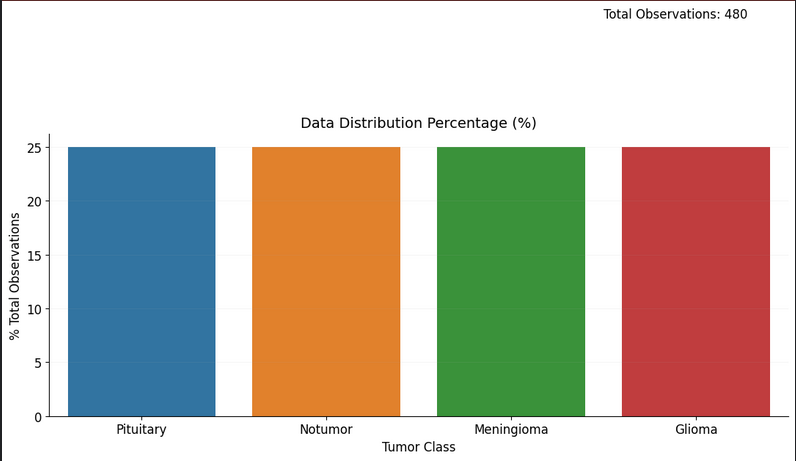
\includegraphics[width=0.75\textwidth]{Exploration/data_distribution.png}
  \end{center}
  \caption{Distribution of images in \texttt{dataset\_19}.}\label{fig:data_distribution}
\end{figure}

Overall, \texttt{dataset\_19} provides a diverse and balanced set of images, essential for training an accurate and reliable deep learning model. The inclusion of different tumor types and multiple views per case enriches the dataset, making it a valuable resource for the task of brain tumor classification.

\subsection{Tumor Types}\label{tumor_types}

The dataset encompasses four distinct classes of brain tumors, each representing a unique type of pathology. A thorough understanding of these tumor types is vital for developing a model capable of accurately classifying them.

\begin{figure}[H]
  \begin{center}
    \includegraphics[width=0.2\textwidth]{Exploration/glioma/axial.jpg}
    \includegraphics[width=0.2\textwidth]{Exploration/glioma/coronal.jpg}
    \includegraphics[width=0.2\textwidth]{Exploration/glioma/sagittal.jpg}
  \end{center}
  \caption{Glioma Tumor: Axial, Coronal, and Sagittal Views.}\label{fig:glioma_views}
\end{figure}

Gliomas are the most prevalent primary brain tumors, originating in the glial cells of the brain. These tumors can be further classified into subtypes such as astrocytoma, oligodendroglioma, and glioblastoma. Gliomas are characterized by their infiltrative nature and high recurrence rates, often presenting with varying shapes and irregular borders. The complexity and variability in glioma morphology make them particularly challenging to classify, underscoring the importance of incorporating detailed MRI views to capture their diverse appearances \cite{abd-ellah_automatic_2024}.

\begin{figure}[H]
  \begin{center}
    \includegraphics[width=0.2\textwidth]{Exploration/malignoma/axial.jpg}
    \includegraphics[width=0.2\textwidth]{Exploration/malignoma/coronal.jpg}
    \includegraphics[width=0.2\textwidth]{Exploration/malignoma/sagittal.jpg}
  \end{center}
  \caption{Malignoma Tumor: Axial, Coronal, and Sagittal Views.}\label{fig:malignoma_views}
\end{figure}


Meningiomas, on the other hand, are typically benign tumors arising from the meninges, the protective layers surrounding the brain and spinal cord. These tumors are usually slow-growing and well-defined, which often makes them easier to surgically remove compared to other types. The well-defined nature of meningiomas benefits from clear imaging perspectives, which assist in their precise identification and classification.

\begin{figure}[H]
  \begin{center}
    \includegraphics[width=0.2\textwidth]{Exploration/pituitary/axial.jpg}
    \includegraphics[width=0.2\textwidth]{Exploration/pituitary/coronal.jpg}
    \includegraphics[width=0.2\textwidth]{Exploration/pituitary/sagittal.jpg}
  \end{center}
  \caption{Pituitary Tumor: Axial, Coronal, and Sagittal Views.}\label{fig:pituitary_views}
\end{figure}

Pituitary tumors develop in the pituitary gland, a small but crucial organ located at the base of the brain. These tumors can be either benign or malignant. Given the pituitary gland's critical role in hormone regulation, accurate identification of pituitary tumors is essential. Detailed MRI views help in assessing the tumor's impact on the surrounding brain structures and the gland itself.

\begin{figure}[H]
  \begin{center}
    \includegraphics[width=0.2\textwidth]{Exploration/notumor/axial.jpg}
    \includegraphics[width=0.2\textwidth]{Exploration/notumor/coronal.jpg}
    \includegraphics[width=0.2\textwidth]{Exploration/notumor/sagittal.jpg}
  \end{center}
  \caption{No Tumor: Axial, Coronal, and Sagittal Views.}\label{fig:notumor_views}
\end{figure}

Lastly, the class labeled `No Tumor' includes images of the brain without any detectable tumors. This class is crucial for training the model to accurately distinguish between pathological and non-pathological images, thereby reducing false positives in diagnoses.

In summary, each tumor type in the dataset presents unique challenges and characteristics that must be considered in model development. The inclusion of diverse MRI views, such as axial, coronal, and sagittal perspectives, provides a comprehensive understanding of the tumor morphology and spatial relationships, thereby enhancing the model's ability to accurately classify and differentiate between various brain tumor types.


\subsection{Image Sizes}\label{image_sizes}
The overall average size of the images is approximately $[453.36, 450.83]$ pixels. The smallest image size is $(198, 150)$ pixels, and the largest image size is $(1075, 890)$ pixels. The mean, median, and mode sizes across the dataset are consistent at $[512, 512]$ pixels, suggesting a central tendency around these dimensions.


\begin{figure}[H]
  \begin{center}
    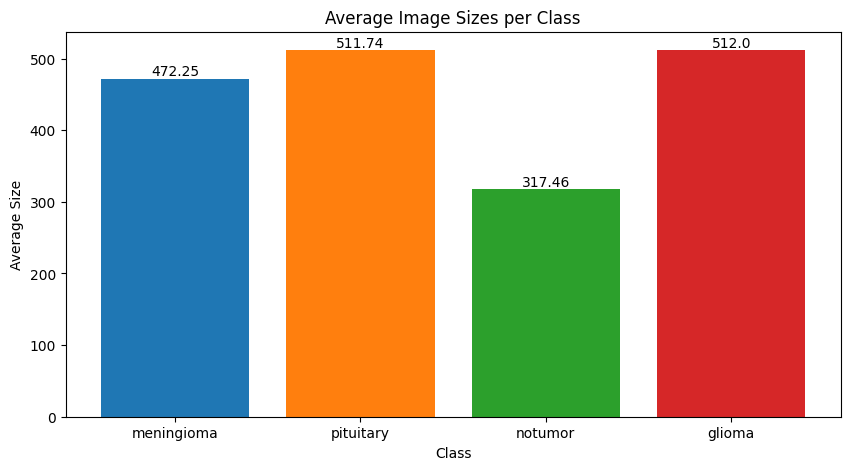
\includegraphics[width=0.75\textwidth]{Exploration/data_sizes.png}
  \end{center}
  \caption{Distribution of brain image sizes in dataset\_19.}\label{fig:data_sizes}
\end{figure}

\begin{longtable}{|l|c|c|}
\caption{Overall Statistics of Brain Image Sizes}\\
\hline
\textbf{Statistic} & \textbf{X} & \textbf{Y} \\
\hline
\endfirsthead
\hline
\textbf{Statistic} & \textbf{X} & \textbf{Y} \\
\hline
\endhead
\hline
\endfoot
\endlastfoot
\textbf{Mean Size} & 453.3625 & 450.83125 \\
\hline
\textbf{Median Size} & 512 & 512 \\
\hline
\textbf{Mode Size} & 512 & 512 \\
\hline
\textbf{Standard Deviation of Size} & 124.1067 & 131.5980 \\
\hline
\textbf{Variance of Size} & 15402.4644 & 17318.0236 \\
\hline
\textbf{Smallest Size} & 198 & 150 \\
\hline
\textbf{Largest Size} & 1075 & 890 \\
\hline
\end{longtable}

\vspace{1cm}

\begin{longtable}{|l|c|c|c|c|}
\caption{Class-Specific Statistics of Brain Image Sizes}\\
\hline
\textbf{Statistic} & \textbf{Meningioma} & \textbf{Pituitary} & \textbf{Notumor} & \textbf{Glioma} \\
\hline
\endfirsthead
\hline
\textbf{Statistic} & \textbf{Meningioma} & \textbf{Pituitary} & \textbf{Notumor} & \textbf{Glioma} \\
\hline
\endhead
\hline
\endfoot
\endlastfoot
\textbf{Mean Size (X)} & 472.25 & 511.7417 & 317.4583 & 512 \\
\hline
\textbf{Mean Size (Y)} & 466.4083 & 510.5417 & 314.3750 & 512 \\
\hline
\textbf{Median Size (X)} & 512 & 512 & 236 & 512 \\
\hline
\textbf{Median Size (Y)} & 512 & 512 & 236 & 512 \\
\hline
\textbf{Mode Size (X)} & 512 & 512 & 236 & 512 \\
\hline
\textbf{Mode Size (Y)} & 512 & 512 & 236 & 512 \\
\hline
\textbf{Standard Deviation of Size (X)} & 100.7078 & 43.5696 & 154.5843 & 0 \\
\hline
\textbf{Standard Deviation of Size (Y)} & 108.4743 & 30.7834 & 174.3213 & 0 \\
\hline
\textbf{Variance of Size (X)} & 10142.0708 & 1898.3083 & 23896.3149 & 0 \\
\hline
\textbf{Variance of Size (Y)} & 11766.6749 & 947.6149 & 30387.9010 & 0 \\
\hline
\textbf{Smallest Size (X)} & 223 & 256 & 198 & 512 \\
\hline
\textbf{Smallest Size (Y)} & 200 & 256 & 150 & 512 \\
\hline
\textbf{Largest Size (X)} & 650 & 903 & 1075 & 512 \\
\hline
\textbf{Largest Size (Y)} & 591 & 721 & 890 & 512 \\
\hline
\end{longtable}

Class-specific statistics reveal a notable variation in image sizes. For the \textit{meningioma} class, image sizes range from $(223, 200)$ to $(650, 591)$ pixels, with a mean size of approximately $[472.25, 466.41]$ pixels. The \textit{pituitary} class exhibits sizes from $(256, 256)$ to $(903, 721)$ pixels, with a mean size of around $[511.74, 510.54]$ pixels. The \textit{notumor} class has sizes ranging from $(198, 150)$ to $(1075, 890)$ pixels, and a mean size of approximately $[317.46, 314.38]$ pixels. In contrast, all images in the \textit{glioma} class are consistently sized at $[512, 512]$ pixels.

This variability in image sizes across different classes underscores the importance of size normalization during the preprocessing phase. While the \textit{glioma} class images are uniformly sized, other classes exhibit significant variation. If not properly addressed, this could introduce biases or inconsistencies in the training process.

Proper preprocessing, including size normalization, is vital for several reasons. Firstly, neural networks require inputs of a fixed size, and resizing is essential to facilitate batch processing of images. Secondly, ensuring all images are of the same size guarantees consistent feature representation across the dataset, aiding in better model learning. Additionally, smaller, consistent image sizes can significantly reduce computational load and memory requirements, thus making training more efficient. Lastly, properly preprocessed images can lead to improved model convergence and accuracy, as the network can learn from a standardized set of inputs.

It is important to note that the image size fed into each model will differ, as each pretrained model is trained on different image sizes. This will be further elaborated in subsequent sections. In conclusion, resizing images to a uniform dimension during the preprocessing step is a critical consideration in developing a robust and efficient deep learning model for brain tumor classification. This step not only facilitates smooth training but also contributes to the overall performance and generalization capability of the model.

